
% this file is called up by thesis.tex
% content in this file will be fed into the main document

% ----------------------- introduction file header -----------------------
%\chapter{Search for the FCNC decay \pmb{$t\rightarrow c + Z$}}
%\chapter{Search for FCNC $t\rightarrow Zc$ without a charm-tagger}
%\label{chapter:regions}

% the code below specifies where the figures are stored
\graphicspath{Chapters/CH7/figures}

% ----------------------------------------------------------------------
% ----------------------- introduction content -------------------------
% ----------------------------------------------------------------------
%This chapter presents the Signal Regions dedicated to the search for FCNC \tZc in \ttbar decays and single-top production without a charm tagger.
%Background sources are also described, as well as the definitions of several Control Regions.

\section{Additional Signal Regions}
\label{sec:selection_all}
The previous sections described the event selection targeting the FCNC \ttbar decay process using a charm-tagger. Without the use of a charm-tagger, two addition selections can be investigated: FCNC \ttbar decays and FCNC single top production.\\
%This two Signal Regions allow the extraction of the FCNC \tzq (q=u,c) limit since they don't use an explicit \Pqc-tagging algorithm. However, performing a likelihood fit using 
The pre-selection criteria, common to all the Signal Regions used in this work have already been discussed in \Cref{sec:selection}.
In this section, the topology of the final states of the signal in the Signal Regions are described. 
For SR3\tZc, the selection using \DLrc and presented in \Cref{sec:other_selection}, is used henceforth.
%The SR3\tZc selection using the \Pqc-tagger \DLrc is already presented in \Cref{sec:other_selection}.
There are two more channels that remain to be presented.
\vspace{\baselineskip}
\\The first selection is \FCNCtZc in \ttbar decays, where one of the \Pqt-quarks decays following the SM into a \PW boson and a
\Pqb-quark %(called in the following \textit{SM top}), while the other
%\Pqt-quark (called in the following \textit{FCNC top}) decays into a \PZ
%boson and a \Pqc-quark. Only the
%trileptonic channel is considered, i.e. when the \PZ boson from the
%FCNC top decays leptonically and the \PW boson from the SM top
%decays leptonically. Therefore the final state is characterised by
%the presence of three leptons, a \Pqc-jet, a \Pqb-tagged jet and missing
%transverse momentum from the escaping neutrino.  
The final state of this channel was already presented in \Cref{sec:selection}  with the exception that no SMT or \Pqc-tagged jet is required.
\vspace{\baselineskip}
\\The second selection is \FCNCtZc in single-top production, where the
production of a single top-quark proceeds through an FCNC
interaction. The \Pqt-quark is produced in association with a \PZ
boson. Also in this case, only the trileptonic channel is
considered. Therefore the final state is characterised by
the presence of three leptons, a \Pqb-tagged jet and missing
transverse momentum from the escaping neutrino. 

\subsection{SR1\tZc selections}
\label{sec:sel:sr1}
The SR1\tZc has the following additional requirements:
\begin{itemize}
	\item At least two jets satisfying the requirements described in 
	\Cref{sec:object:jet}. 
	\item Exactly one \Pqb-jet satisfying the requirements
	described in \Cref{sec:object:bjet}. 
	\item The mass of the FCNC top-quark candidate,
	\mtopfcnc, must be within $2\sigma^{FCNC}$ from \mtopvalue, while no
	requirement on the mass of the SM top-quark candidate, \mtopsm, is applied.
	\item A veto is applied on the events where there is a \Pqc-tagged jet, described in~\Cref{sec:object:cjet}.
\end{itemize}
Kinematic plots are presented in Appendix~\ref{app:SRs:SR1}.

% -------------------------------------------------------------------------------
\subsection{SR2\tZc selections}
\label{sec:sel:sr2}

The SR2\tZc has the following additional requirements:
\begin{itemize}
	\item Exactly one or two jets satisfying the requirements described in 
	\Cref{sec:object:jet}. 
	\item Exactly one \Pqb-jet satisfying the requirements
	described in \Cref{sec:object:bjet}. 
	\item The lepton not used to reconstruct the \PZ boson is assumed to be
	the one coming from the \PW boson.
	The transverse mass is calculated using the momentum of the lepton associated with the $W$ boson, $\MET$ and azimuthal angle,$\phi$, between them: 
	$\mT(\ell_{\PW},\Pgn) = \sqrt{2\pT^{\ell}\MET \left(1-\cos\Delta\phi\right)}$.
	Events are required to have $\mT(\ell_{\PW},\Pgn) > \SI{40}{\GeV}$.
	\item For events with exactly one jet, no
	requirement is applied on the masses of the FCNC and SM top-quark
	candidates. For events with exactly two jets, the mass of the FCNC
	top-quark candidate, \mtopfcnc, must be outside $2\sigma^{FCNC}$
	from \mtopvalue, while the mass of the SM top-quark candidate,
	\mtopsm, must be within $2\sigma^{SM}$ from \mtopvalue. The
	requirement on \mtopfcnc makes this region orthogonal to SR1.
	\item A veto is applied on the events where there is a \Pqc-tagged jet, described in~\Cref{sec:object:cjet}.
\end{itemize}
Kinematic plots are presented in Appendix~\ref{app:SRs:SR2}.

\subsection{Orthogonality between Signal Regions}
The SRs are orthogonal between each other. The orthogonality is assured by
selecting events with different jet multiplicities, by selecting or vetoing the presence of c-tagged jet and selecting different mass windows using the reference value for the top mass of \mtopvalue. The mass windows applied are much larger than the difference between \mtopvalue and the mass values extracted in Appendix \ref{appendix:mass_resolution} and used in the $\chi^{2}$ calculation (see \Cref{eq:chi2tt,eq:chi2tZ}). Therefore, changing the mass value would not have a significant effect on the number of events in the SRs. Moreover, it is better to keep the mass window larger as possible to have a high signal sensitivity.\\
This can be verified in Table~\ref{tab:sel:srs} where an overview of the requirements applied to select 
events in the Signal Regions is presented.

\clearpage
%\global\pdfpageattr\expandafter{\the\pdfpageattr/Rotate 90}
\begin{sidewaystable}[!htbp]
	\centering
	\begin{tabular}{c|c|c|c}
		\toprule
		\multicolumn{4}{c}{Common selections} \\
		\midrule
		\multicolumn{4}{c}{Exactly 3 leptons with $|\eta| < 2.5$ and $\pT(\ell_1)> \SI{27}{\GeV}$, $\pT(\ell_2)> \SI{15}{\GeV}$, $\pT(\ell_3)> \SI{15}{\GeV}$} \\
		\multicolumn{4}{c}{$\ge$ 1 \OSSF pair, with $|\mll - \SI{91.2}{\GeV}| < \SI{15}{\GeV}$} \\
		% \multicolumn{4}{c}{$\mT(\ell_{\PW},\Pgn) > \SI{40}{\GeV}$} \\
		% \multicolumn{4}{c}{$\pT(\text{jet})> \SI{35}{\GeV}$} &  \\
		\midrule
		\midrule
		SR1\tZc & \multicolumn{2}{c|}{SR2\tZc} & SR3\tZc \\
		\midrule 
		$\ge$ 2 jets with $|\eta| < $ 2.5  & = 1 jet with $|\eta| < $ 2.5  & = 2 jets with $|\eta| < $ 2.5  & $\ge$ 2 jets with $|\eta| < $ 2.5 \\
		= 1 \Pqb-jet  & = 1 \Pqb-jet & = 1 \Pqb-jet & = 1 \Pqb-jet \\
		-- & $\mT$($\ell_{\PW},\Pgn$)$ > \SI{40}{\GeV}$ & $\mT$($\ell_{\PW},\Pgn$)$ > \SI{40}{\GeV}$ & -- \\
		% --  & -- & -- & OS($\mu^{soft}$,$\ell_W$) & OS($\mu^{soft}$,$\ell_W$) \\
		% = 0 SMT anti-\Pqb-tagged jet  & -- & = 0 SMT anti-\Pqb-tagged jet & $\ge$ 1 SMT anti-\Pqb-tagged jet & $\ge$ 1 SMT \Pqb-tagged jet\\
		= 0 \Pqc-tagged jet  & -- & = 0 \Pqc-tagged jet & $\ge$ 1 \Pqc-tagged jet \\
		$|\mtopfcnc - \mtopvalue| < 2\sigma^{FCNC}$ & -- & $|\mtopfcnc - \mtopvalue| > 2\sigma^{FCNC}$ & -- \\
		-- & -- & $|\mtopsm - \mtopvalue| < 2\sigma^{SM}$ & -- \\
		\bottomrule
	\end{tabular}
	\caption{
	Overview of the requirements applied to select events in the Signal Regions.
}%
\label{tab:sel:srs}
\end{sidewaystable}
\clearpage
\FloatBarrier
%\global\pdfpageattr\expandafter{\the\pdfpageattr/Rotate 0}


\subsection{Event yields in the Signal Regions}
Event yields in the SRs for the \tZc coupling extraction are reported in Table~\ref{tab:sel:yields:tzc}.\\
The SR1 and SR2 have been presented before (in \Cref{sec:sel:sr1} and \Cref{sec:sel:sr2} respectively),
while for SR3, as demonstrated in \Cref{sec:other_selection}, the selection using the charm-tagger \DLrc
w.r.t. SMT, provided the best \ssplusb ratio for this analysis and then it is exploited in the following.\\
As it can be noticed, the main background sources are:
\begin{itemize}
	\item for SR1\tZc, \ttZ and \VVHF;
	\item for SR2\tZc, \VVHF and Standard Model \tZq ;
	\item for SR3\tZc, \ttZ and \VVHF .
\end{itemize}

\begin{table}[!htbp]
	\centering
	\small
	% NB: add to main document: 
% \usepackage{siunitx} 
% \sisetup{separate-uncertainty,table-format=6.3(6)}  % hint: modify table-format to best fit your tables
\begin{tabular}{|p{0.18\textwidth}|>{\centering}p{0.21\textwidth}|>{\centering}p{0.2\textwidth}|>{\centering\arraybackslash}p{0.2\textwidth}|}
\toprule  
 & {SR1tZc} & {SR2tZc} & {SR3tZc}\\
\midrule 
 \ttZ   & 137.9 $\pm$ 0.9 & 24.11 $\pm$ 0.31 & 69.5 $\pm$ 0.6 \\ 
\tWZ   & 30.6 $\pm$ 0.8 & 9.4 $\pm$ 0.4 & 12.4 $\pm$ 0.5 \\ 
\ttW   & 5.78 $\pm$ 0.22 & 3.33 $\pm$ 0.15 & 2.04 $\pm$ 0.12 \\ 
\ttH   & 6.10 $\pm$ 0.08 & 0.881 $\pm$ 0.023 & 2.63 $\pm$ 0.05 \\ 
\VVLF   & 28.2 $\pm$ 0.5 & 34.8 $\pm$ 1.5 & 2.89 $\pm$ 0.14 \\ 
\VVHF   & 142.7 $\pm$ 1.0 & 155.9 $\pm$ 2.2 & 30.3 $\pm$ 0.4 \\ 
\tZq   & 46.5 $\pm$ 0.6 & 110.0 $\pm$ 0.7 & 13.82 $\pm$ 0.28 \\ 
\ttbar   & 20.0 $\pm$ 0.9 & 31.5 $\pm$ 1.1 & 3.7 $\pm$ 0.4 \\ 
\Wt   & 0.7 $\pm$ 0.4 & 0.8 $\pm$ 0.4 & <\:0.001 \\ 
\Zjets   & 9.9 $\pm$ 1.6 & 11.8 $\pm$ 1.9 & 1.3 $\pm$ 0.6 \\ 
\VH   & 1.2 $\pm$ 1.2 & 3.2 $\pm$ 1.2 & <\:0.001 \\ 
\ttWW   & 0.39 $\pm$ 0.06 & 0.027 $\pm$ 0.016 & 0.16 $\pm$ 0.04 \\ 
\VVV   & 0.704 $\pm$ 0.032 & 0.590 $\pm$ 0.034 & 0.220 $\pm$ 0.016 \\ 
4 tops   & 0.151 $\pm$ 0.011 & 0.0030 $\pm$ 0.0012 & 0.092 $\pm$ 0.010 \\ 
3 tops   & 0.0220 $\pm$ 0.0029 & 0.0011 $\pm$ 0.0010 & 0.0155 $\pm$ 0.0025 \\ 
\ttZ (2l)   & 0.046 $\pm$ 0.034 & 0.009 $\pm$ 0.029 & 0.02 $\pm$ 0.05 \\ 
\VV (2l)   & 0.49 $\pm$ 0.12 & 0.30 $\pm$ 0.11 & 0.05 $\pm$ 0.07 \\ 
FCNC (c)tZ   & 3.24 $\pm$ 0.06 & 11.81 $\pm$ 0.10 & 1.205 $\pm$ 0.033 \\ 
FCNC \ttbar(cZ)   & 57.3 $\pm$ 0.6 & 17.67 $\pm$ 0.33 & 21.9 $\pm$ 0.4 \\ 
\midrule 
Total background  & 431.4 $\pm$ 2.7 & 387 $\pm$ 4 & 139.1 $\pm$ 1.2 \\ 
\bottomrule 
\end{tabular} 

	\caption{Event yields in the SRs for the \tZc coupling extraction. \TabErrStatOnly} 
	\label{tab:sel:yields:tzc}
\end{table} 
\noindent As expected, SR1 has the greater fraction of FCNC \ttbar(cZ) events because it is designed to target the decay signal topology, while SR2 has the greater fraction of FCNC (c)tZ events because it is designed to target the FCNC single top production.\\
The signal yield in SR3 is affected by the \DLrc  \Pqc-efficiency (20\%), as discussed in~\Cref{sec:object:cjet} but it also has the best background rejection. However, SR1 cannot distinguish between $\mathrm{\Pqt\rightarrow\PZ\Pqu}$ and $\mathrm{\Pqt\rightarrow\PZ\Pqc}$ as no c-tagger is used in this region and the choice of the jet coming from the FCNC top decay is defined by the $\chi^2$ minimization.

\clearpage
\section{Background estimation}
\label{sec:background_all}
A variety of background sources are considered and already discussed in \Cref{sec:background}.\\
In order to improve the modelling of the main background processes, Control Regions (CRs) are used in the fit to extract the normalisation of some relevant background sources.\\
Several CRs are defined:
\begin{itemize}
	\item \ttbar CR is designed to control the minor \ttbar
	background. As previously mentioned, this background enters the
	selection because of the presence of a mis-reconstructed lepton,
	i.e. a fake lepton. Since this background is small, the decision was
	taken to evaluate it using MC simulations. Nevertheless, the normalisation is
	taken from data because these events are considered fakes for this analysis.. 
	\item \ttZ CR is designed to control the \ttZ
	background. It is constructed by requiring the presence of more jets
	with respect to the jet multiplicity required in the SRs.
	\item Side-band CRs are designed to contain a mixture
	of the main background sources (\ttZ and diboson). They are
	constructed reversing the SR cuts on the top masses.
\end{itemize}

\subsection {Control Regions definition}
\label{sec:bkg:sel}
In the following, the event selection in the CRs is described.\\
\Cref{tab:bkg:crs} summarises the selection cuts in the various CRs.
\paragraph{\ttbar CR selections}
The \ttbar CR is defined by requiring that there is at least one pair
of opposite-sign but different-flavour leptons in the
event. No cut on the invariant mass of the opposite-sign
leptons is applied. Concerning the jet multiplicity, there should be
at least one jet in the event, of which exactly one should be
\Pqb-tagged. Kinematic plots are presented in Appendix~\ref{app:CRs:tt}.

\paragraph{\ttZ CR selections}
\label{sec:bkg:ttz}
The \ttZ CR is defined by requiring the presence of at least four jets
of which exactly two \Pqb-tagged. Also the cut on the transverse
mass of the \PW boson is softened to \SI{30}{\GeV}. To be orthogonal 
with SR3\tZc, also a veto on the presence of a \Pqc-jet is required. 
Kinematic plots are presented in Appendix~\ref{app:CRs:ttZ}.

\paragraph{Side-band CR1 selections}
\label{sec:bkg:sbcr1tzu}
The mass side-band CR1 is defined by requiring the presence of at least two jets
and of exactly one \Pqb-tagged jet.
The mass of the FCNC top-quark candidate, \mtopfcnc,
must be outside $2\sigma^{FCNC}$ from \mtopvalue, the mass of the
SM top-quark candidate, \mtopsm, must be also outside $2\sigma^{SM}$
from \mtopvalue.  In addition, a veto on the presence of a \Pqc-jet is required. 
Kinematic plots are presented in Appendix~\ref{app:CRs:SB1}.

\paragraph{Side-band CR2 selections}
\label{sec:bkg:sbcr2}
The mass side-band CR2 is defined by requiring the presence of exactly one or two jets
and of exactly one \Pqb-tagged jet.  
Events are required to have $\mT(\ell_{\PW},\Pgn) > \SI{40}{\GeV}$.\\
The mass of the SM top-quark candidate, \mtopsm, must be also outside $2\sigma^{SM}$
from \mtopvalue. Kinematic plots are presented in Appendix~\ref{app:CRs:SB2}.

\clearpage
%\global\pdfpageattr\expandafter{\the\pdfpageattr/Rotate 90}
\begin{sidewaystable}[!htbp]
	\centering
	\footnotesize
	\begin{tabular}{c|c|c|c}
		\toprule
		\multicolumn{4}{c}{Common selections} \\
		\midrule
		\multicolumn{4}{c}{Exactly 3 leptons with $|\eta| < 2.5$ and $\pT(\ell_1)> \SI{27}{\GeV}$, $\pT(\ell_2)> \SI{15}{\GeV}$, $\pT(\ell_3)> \SI{15}{\GeV}$} \\
		\midrule
		\ttbar CR & \ttZ CR & Side-band CR1 & Side-band CR2 \\
		\midrule
		$\ge$ 1 \OS pair, no \OSSF  & $\ge$ 1 \OSSF pair & $\ge$ 1 \OSSF pair & $\ge$ 1 \OSSF pair \\
		& with $|\mll - \SI{91.2}{\GeV}| < \SI{15}{\GeV}$ & with $|\mll - \SI{91.2}{\GeV}| < \SI{15}{\GeV}$ & with $|\mll - \SI{91.2}{\GeV}| < \SI{15}{\GeV}$ \\
		-- & $\mT(\ell_{\PW},\Pgn) > \SI{30}{\GeV}$ & $\mT(\ell_{\PW},\Pgn) > \SI{40}{\GeV}$ & $\mT(\ell_{\PW},\Pgn) > \SI{40}{\GeV}$ \\
		$\ge$ 1 jet with $|\eta| < $ 2.5  & $\ge$ 4 jet with $|\eta| < $ 2.5 & $\ge$ 2 jet with $|\eta| < $ 2.5  & = 1 jet with $|\eta| < $ 2.5 \\
		= 1 \Pqb-jet  & = 2 \Pqb-jet  &  = 1 \Pqb-jet & = 1 \Pqb-jet \\
		-- & -- & = 0 \Pqc-jet & --\\ 
		-- & -- &  $|\mtopfcnc - \mtopvalue| > 2\sigma^{FCNC}$ & -- \\
		-- & -- & $|\mtopsm - \mtopvalue| > 2\sigma^{SM}$ & $|\mtopsm - \mtopvalue| > 2\sigma^{SM}$ \\
		\bottomrule
	\end{tabular}
	\caption{
		Overview of the requirements applied to select events in the control regions.
	}%
	\label{tab:bkg:crs}
\end{sidewaystable} 
\clearpage
\FloatBarrier
%\global\pdfpageattr\expandafter{\the\pdfpageattr/Rotate 0}

\clearpage


\subsection{Event yields in the Control Regions}
Event yields in the CRs are shown in \Cref{tab:bkg:yields:tzc}. 
As it can be noticed, the signal contribution in the various CRs is small.
Every Control Region is enriched of the correspondent background. 
\begin{table}[htbp]
	\footnotesize
	\centering
	% NB: add to main document: 
% \usepackage{siunitx} 
% \sisetup{separate-uncertainty,table-format=6.3(6)}  % hint: modify table-format to best fit your tables
\begin{tabular}{|p{0.16\textwidth}|>{\centering}p{0.16\textwidth}|>{\centering}p{0.16\textwidth}|>{\centering}p{0.16\textwidth}|>{\centering\arraybackslash}p{0.16\textwidth}|}
\toprule  
 & {Side-band CR1} & {Side-band CR2} & {\ttZ CR} & {\ttbar CR}\\
\midrule 
 \ttZ+\tWZ   & 88 $\pm$ 12 & 9.1 $\pm$ 2.1 & 164 $\pm$ 22 & 14.8 $\pm$ 1.9 \\ 
\ttW   & 4.3 $\pm$ 0.7 & 2.5 $\pm$ 0.5 & 2.3 $\pm$ 0.5 & 27 $\pm$ 4 \\ 
\ttH   & 2.3 $\pm$ 0.4 & 0.36 $\pm$ 0.07 & 5.4 $\pm$ 0.9 & 13.8 $\pm$ 2.1 \\ 
\VVLF   & 25 $\pm$ 15 & 18 $\pm$ 7 & 0.20 $\pm$ 0.22 & 0.40 $\pm$ 0.21 \\ 
\VVHF   & 130 $\pm$ 80 & 69 $\pm$ 28 & 13 $\pm$ 11 & 2.3 $\pm$ 1.4 \\ 
\tZq   & 20 $\pm$ 4 & 9.9 $\pm$ 1.7 & 14.6 $\pm$ 2.9 & 0.90 $\pm$ 0.15 \\ 
\ttbar+Wt   & 10 $\pm$ 4 & 9.1 $\pm$ 2.7 & 3.0 $\pm$ 1.2 & 102 $\pm$ 24 \\ 
Other fakes   & 3 $\pm$ 5 & 10 $\pm$ 11 & 0.00 $\pm$ 0.06 & 0.12 $\pm$ 0.14 \\ 
Other   & 2.2 $\pm$ 1.6 & 0.8 $\pm$ 2.6 & 1.1 $\pm$ 0.5 & 2.9 $\pm$ 1.5 \\ 
\midrule 
Total background  & 280 $\pm$ 80 & 130 $\pm$ 32 & 203 $\pm$ 27 & 164 $\pm$ 25 \\ 
\midrule 
Data   & 331 & 169 & 197 & 156 \\ 
\midrule 
Data / Bkg.   & 1.18 $\pm$ 0.35 & 1.30 $\pm$ 0.34 & 0.97 $\pm$ 0.14 & 0.95 $\pm$ 0.16 \\ 
\bottomrule 
\end{tabular} 

	\caption{Event yields in the CRs for the \tZc coupling extraction. \TabErrStatSys} 
	\label{tab:bkg:yields:tzc}
\end{table} 


\section{Separation of signal from background events using \DLrc}
\label{sec:separation_all}
Three different GBDTs are trained separately in each signal region.
In this section only the GBDT for SR3\tZc will be presented because it is directly related to the work of this thesis.\\
The SR3\tZc is defined targeting the FCNC \tZc coupling in \ttbar decay events using the charm tagger \DLrc, therefore the MVA discriminant for this coupling, \Dthree, is built using the GBDT trained with the FCNC \tZc \ttbar decay events against backgrounds.\\
The procedure is not different from that described in \Cref{sec:separation} and only the final results will be presented.
The final set of variables used to train and test the GBDT on the events in
SR3\tZc is in \Cref{tab:D3input_dl1rc}, ordered by the separation value.\\
The five GBDT output scores used to built discriminant variables are compared in~\Cref{fig:separation:GBDT_dl1rc}.\\
\begin{table}[!htbp]
	\small
	\centering
	\begin{tabular}{ccc}
		\toprule
		Variable & $\langle s^{2}\rangle$  & Definition \\
		\midrule
		$m_{b\ell\nu}$  &  0.1329  &  SM top-quark candidate mass  \\
		$\pT^{q}$  &  0.07402  &  $u$/$c$-quark candidate transverse momentum  \\
		$N_{jets}$  &  0.0575  &  Jet multiplicity  \\
		$m_{q\ell\ell}$  &  0.04343  &  FCNC top-quark candidate mass  \\
		$\Delta R(t_{\text{SM}},t_{\text{FCNC}})$  &  0.03822  &  $\Delta R$ between SM and FCNC top-quark candidates  \\
		$\Delta R(c,Z)$  &  0.0359  &  $\Delta R$ between $c$-quark and $Z$ boson candidates  \\
		$\Delta R(\ell,Z)$  &  0.02417  &  $\Delta R$ between $W$ boson lepton and $Z$ boson candidates  \\
		\bottomrule
	\end{tabular}
	\caption{ Variables used in the training of the GBDT in SR3\tZc to built the \Dthree discriminant used in \tZc coupling search. Variables are ordered by the separation 	$\langle s^{2}\rangle$ value, already defined in \Cref{sec:input_var}. }%
\label{tab:D3input_dl1rc}
\end{table}

\begin{figure}[!htbp]
	\centering
	\subfigure[]{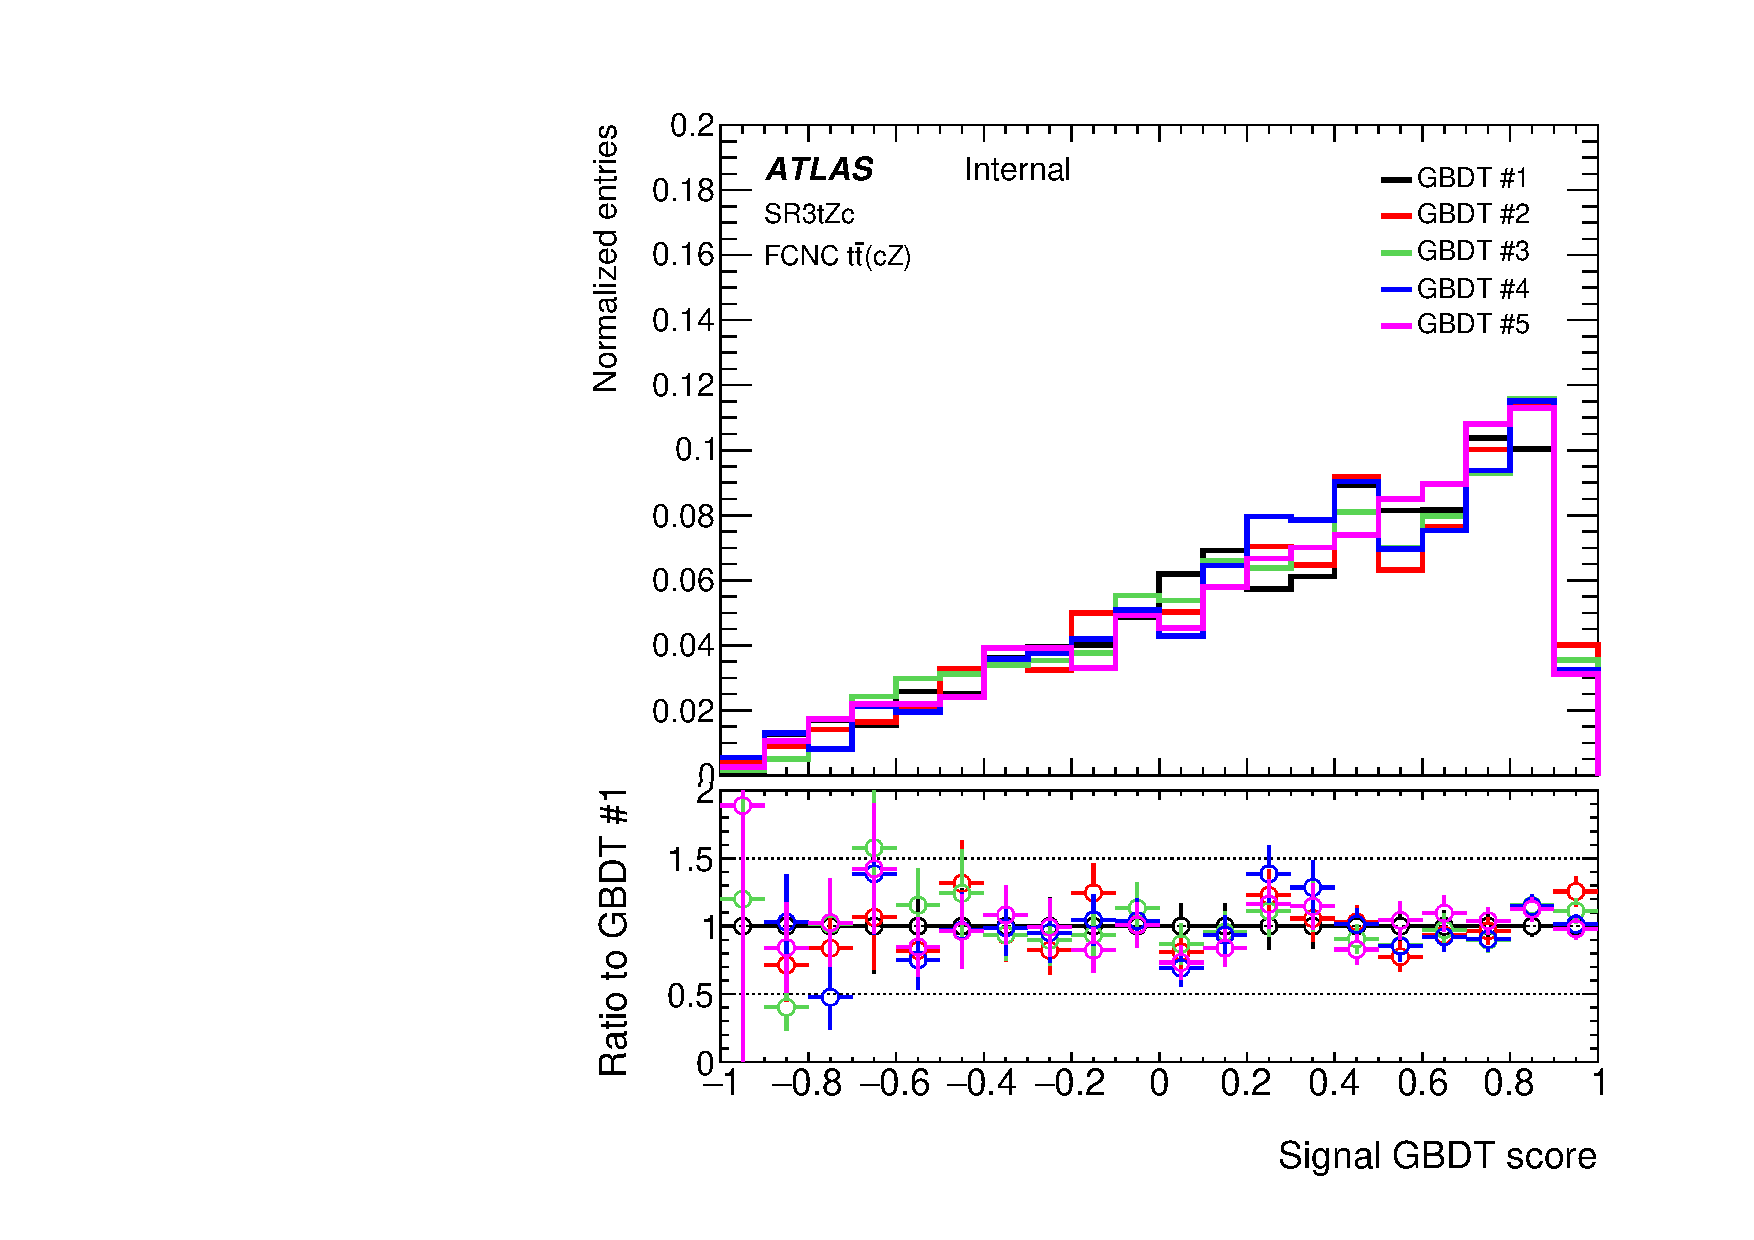
\includegraphics[width=.4\textwidth]{Chapters/CH7/figures/cveto_bdt/GBDT_signal}\label{subfig:separation:GBDTsig_dl1rc}}\qquad
	\subfigure[]{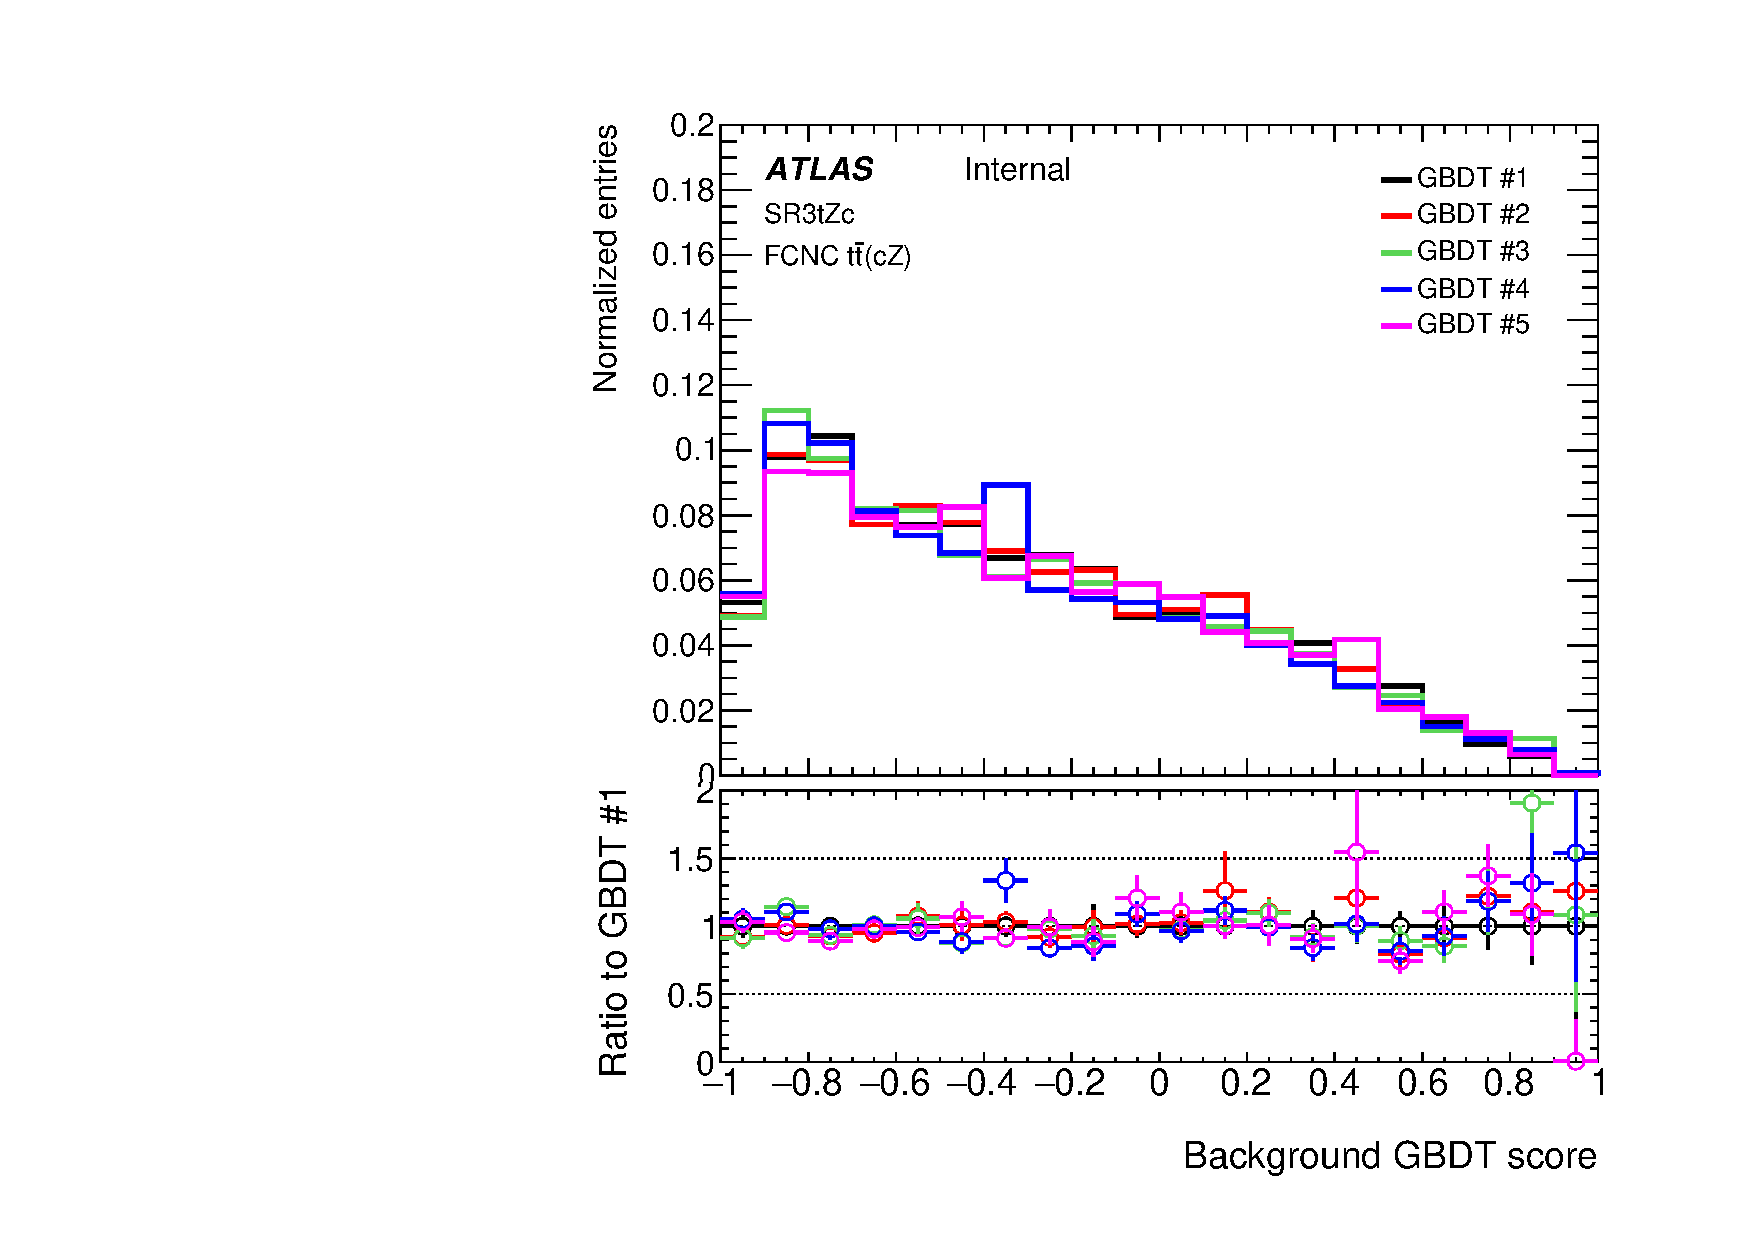
\includegraphics[width=.4\textwidth]{Chapters/CH7/figures/cveto_bdt/GBDT_background}\label{subfig:separation:GBDTbkg_dl1rc}}
	\caption{ The GBDT output score distributions for \subref{subfig:separation:GBDTsig_dl1rc} signal events and \subref{subfig:separation:GBDTbkg_dl1rc} background events, in the test samples. The five trained GBDTs are compared in each signal region.}
	\label{fig:separation:GBDT_dl1rc}
\end{figure}


%
%\begin{table}[htbp]
%	\caption{
%		Summary of the GBDT discriminant variables with their training regions, signal samples and search coupling.
%	}%
%	\label{tab:discriminants}
%	\centering
%	\begin{tabular}{cccc}
%		\toprule
%		GBDT discriminant & Training Region & Training signal & Search coupling \\
%		\hline
%		\Done   & SR1 \tZu & FCNC \tZu and \tZc in \ttbar decays & \tZu, \tZc \\
%		\DtwoU & SR2 \tZu & FCNC \tZu in \tZ production & \tZu \\
%		\DtwoC & SR2 \tZu & FCNC \tZc in \ttbar decays and \tZ production & \tZc \\
%		\Done & SR3 \tZc & FCNC \tZc in \ttbar decays & \tZc \\
%		\bottomrule
%	\end{tabular}
%\end{table}


%\clearpage
%\subsection {Fake composition}
%The origin of the three leptons from \ttbar events was studied, to
%understand where the fake leptons come from and eventually define an
%uncertainty to take into account the different sources in the signal
%and control regions. The origin of the three leptons from \ttbar
%events is shown in \cref{fig:bkg:fakes:ttbar:comp}. As it can be
%seen, apart from the leptons for which the mother is the top quark
%(\SI{66}{\%} of the leptons in each event), the fake leptons come from
%either photon conversions (around \SI{5}{\%}, depending on the region)
%or from \Pqb-hadrons (around \SI{25}{\%}, depending on the region). \\
%Some differences can be noticed for the photon conversion and
%\Pqb-hadron fractions in the signal regions with respect to the \ttbar
%control region where the \ttbar background is controlled. To take into
%account this differences, a systematic uncertainties is added. 
%
%\begin{figure}[htbp]
%	\centering
%	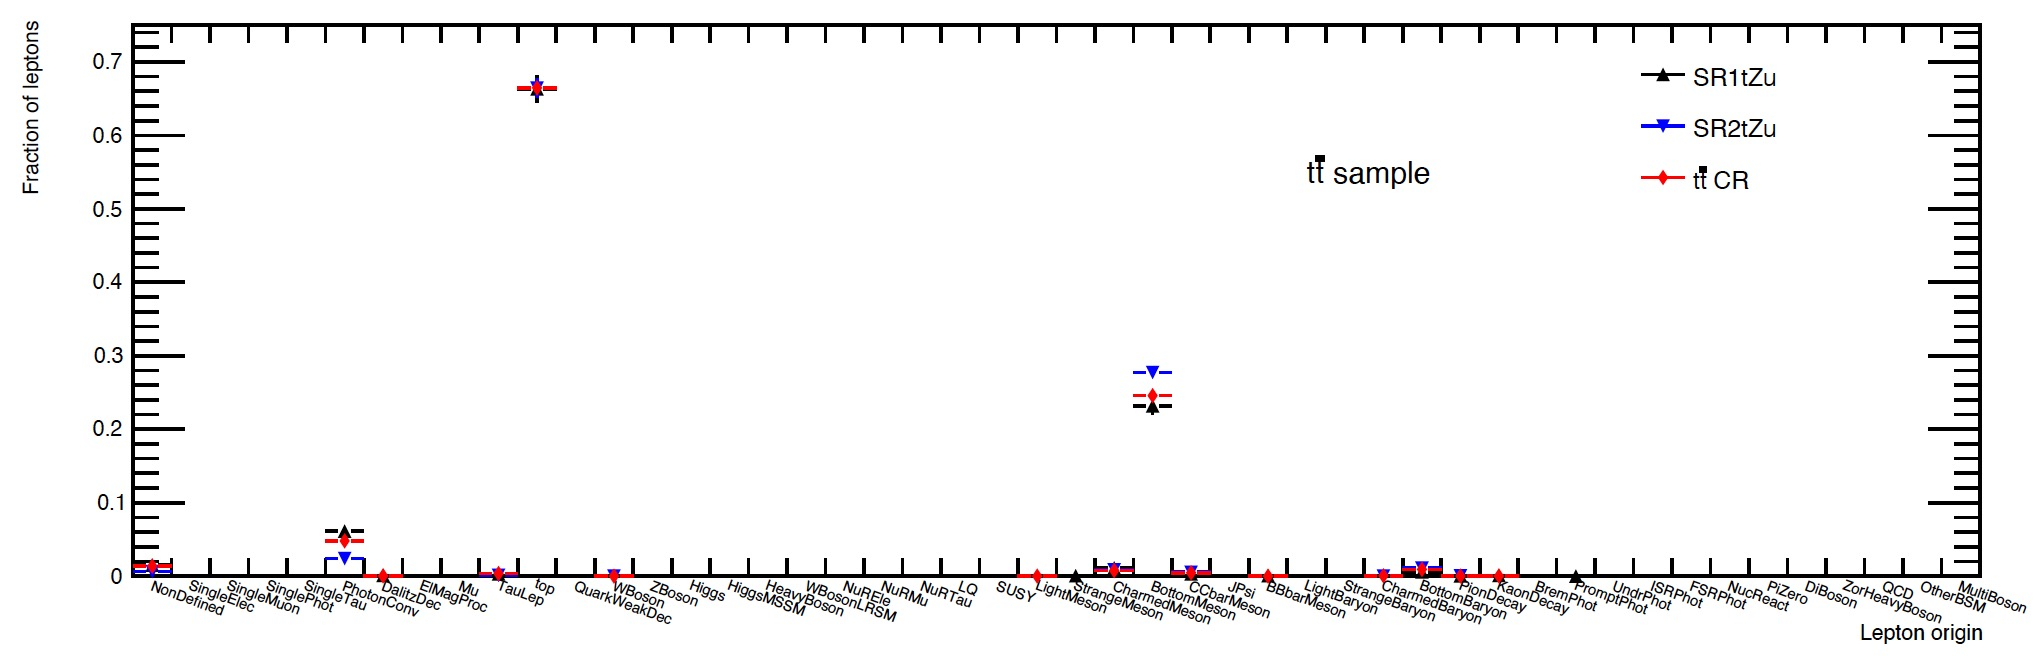
\includegraphics[width=1.\textwidth]{Chapters/CH5/figures/ttbar_leptons_origin}
%	\caption{Origin of the three leptons from \ttbar events in the
%		SR1\tZu, SR2\tZu and \ttbar CR. 
%	}%
%	\label{fig:bkg:fakes:ttbar:comp}
%\end{figure}
%
%\clearpage
%\FloatBarrier

